\section{Signalflussdiagramm \formelbuch{217} \tiny{$Revision: 998 $}}
\begin{list}{$\bullet$}{\setlength{\itemsep}{0cm} \setlength{\parsep}{0cm} \setlength{\topsep}{0cm}} 
  \item Graphische Lösung linearer Gleichungen
  \item Graphische Darstellung von LTI-Systemen
  \item Änderung der Topologie ohne UTF zu ändern
\end{list}

% \subsection{Definition}
% \begin{list}{$\bullet$}{\setlength{\itemsep}{0cm} \setlength{\parsep}{0cm} \setlength{\topsep}{0cm}}
%   \item \textbf{Knoten}: Darstellung einer Grösse, eines Signals oder einer
%   Variable
%   \item \textbf{Zweig}: Funktionelle Abhängigkeit einer Grösse
%   \item \textbf{Quelle}: Unabhängiger Knoten, es münden keine Zweige ein
%   \item \textbf{Senke}: Knoten, ohne weggehende Zweige
%   \item \textbf{Pfad}: Kontinuierliche Folge von Zweigen, die in die gleiche
%   Richtung zeigen
%   \item \textbf{Offener Pfade}: Ein Pfad, bei dem jeder beteiligte Knoten nur einmal durchquert
% wird
%   \item \textbf{Vorwärtspfad}: Ein offener Pfad zwischen einer Quelle und einer
%   Senke
%   \item \textbf{Schleife}: Ein geschlossener Pfad, welcher zum Ausgangsknoten
%   zurückkehrt, wobei jeder beteiligte Knoten nur einmal durchlaufen wird, ausgenommen der
% Ausgangsknoten
%   \item \textbf{Eigenschleife}: Eine (Rückkopplungs)schleife, die aus einem
%   Zweig und einem Knoten besteht
%   \item \textbf{Zweigtransmittanz}: Die lineare Grösse, unabhängig von ihrer
%   Dimension, die einen Knoten eines Zweiges zum anderen Knoten in Beziehung setzt.
%   \item \textbf{Schleifentransmittanz}: Das Produkt der Zweigtransmittanzen in
%   einer Schleife.
% \end{list}

\subsection{Transformationsregeln \formelbuch{223ff.}}

\subsection{Mason's Regel \formelbuch{230}}
$\boxed{T_{ij} = \frac{\sum\limits_k P_k\cdot\Delta_k}{\Delta}}\quad
\Rightarrow$ UTF von $x_i$ nach $x_j$, wobei \textbf{$x_i$} eine
\textbf{Quelle}, \textbf{$x_j$} jedoch nicht zwingend eine \textbf{Senke} sein
muss. \vspace{0.3cm}\\
$P_k \Rightarrow$ Vorwärtspfad $k$ \qquad $\Delta_k \Rightarrow$ Kofaktor de
$k$-ten Pfades \qquad $\Delta \Rightarrow$ Netzwerkdeterminante\vspace{0.3cm}\\
$\Delta$ = 1- (Summe aller Schleifen) + (Summe aller Produkte zweier
Schleifen, die sich nicht berühren) - (Summe
aller Produkte dreier Schleifen, die sich nicht berühren) + $\ldots$
\vspace{0.3cm}\\
$\Delta_k$ = 1- (Summe aller Schleifen die $P_k$ nicht berühren) + (Summe
aller Produkte zweier Schleifen, die $P_k$ und sich selbst nicht
berühren)-(Summe aller Produkte dreier Schleifen, die $P_k$ und sich selbst
nicht berühren) + $\ldots$ \\

Falls die \textbf{UTF eines SFD von einem beliebigen Knoten} (keiner Quelle)
gesucht wird, kann Mason's Regel nicht direkt angewandt werden. Abhilfe: \\
$T_{ij} = \frac{x_j}{x_i} = \frac{x_j}{x_q} \frac{x_q}{x_i} =
\frac{T_{qj}}{T_{qi}}$ Wobei $x_q$ eine Quelle sei. 
Schlussendlich kürzt sich die Netzwerkdeterminante heraus.


\subsection{Beispiel eines SFD \formelbuch{235}}
\begin{tabular}{ll}
	\parbox{7cm}{
    	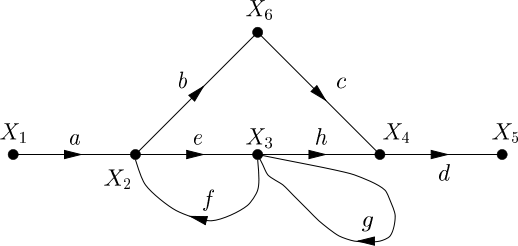
\includegraphics[width=7cm]{./bilder/sfd-bsp.png}
    }
    
    & \parbox{12cm}{
    \begin{enumerate}
		\item[a)] Die UTF\index{UTF} zwischen $X_1$ und $X_4$ ist (mit Mason's Regel):\index{Mason's Regel}\\
		\begin{equation*}
		H_{14}=\frac{X_4}{X_1}=\frac{aeh+abc(1-g)}{1-ef-g}
		\end{equation*}
		\item[b)] Das folgende Gleichungssystem beschreibt das SFD.
		\begin{eqnarray*}
		X_2 &=&a\cdot X_1+f\cdot X_3\\
		X_3 &=&e\cdot X_2+g\cdot X_3\\
		X_4 &=&h\cdot X_3+c\cdot X_6\\
		X_5 &=&d\cdot X_4\\
		X_6 &=&b\cdot X_2
		\end{eqnarray*}
		Nach Umformung der Gleichungen erhalten wir:
		\begin{equation*}
		X_4=h\cdot X_3+\frac{bc}{e}\cdot (1-g)\cdot X_3\quad\&\quad X_3\cdot
		\frac{1-g}{e}=a\cdot X_1+f\cdot X3.
		\end{equation*}
		Somit ist $X_4=\frac{h+\frac{bc}{e}(1-g)}{\frac{1-g}{ae}-\frac{f}{a}}X_1=\frac{aeh+abc(1-g)}{1-g-ef}X_1$.
	\end{enumerate}}
\end{tabular}

\subsection{Fundamentales SFD \formelbuch{236}}
\begin{tabular}{ll}
	\parbox{7cm}{
    	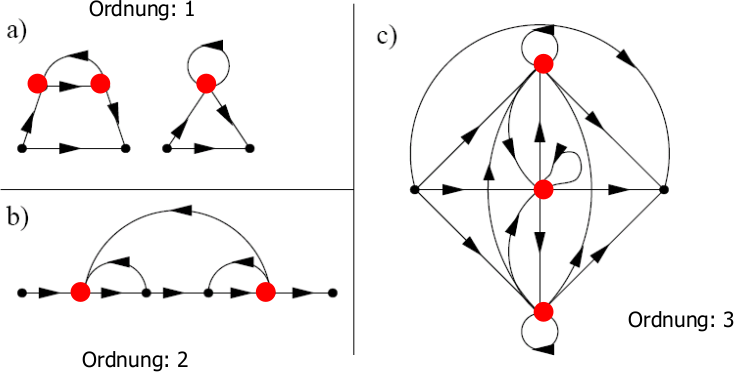
\includegraphics[width=7cm]{./bilder/sfd-ordnung.png}
    }
    
    & \parbox{12cm}{
		\textit{Ordnung eines SFD = Anzahl der fundamentalen Knoten}: Knoten, welche
		entfernt werden müssen, um \textit{alle} Schleifen aufzubrechen. \\ \\
	}
\end{tabular}
\subsubsection{Fundamentales SFD erster Ordnung \formelbuch{237}}
\begin{tabular}{ll}
	\parbox{7cm}{
    	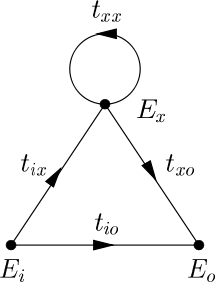
\includegraphics[width=3cm]{./bilder/sfd-fundamental-erster-ordnung.png}
    }
    & \parbox{12cm}{
		Durch Reduzieren auf das fundamentale SFD 1. Ordnung, kann die UTF direkt
		ermittelt werden: \\
		$$\frac{E_o}{E_i}=
		t_{io}+\frac{t_{ix}t_{xo}}{1-t_{xx}}=
		\frac{t_{io}-t_{io}t_{xx}+t_{ix}t_{xo}}{1-t_{xx}}$$
	}
\end{tabular}

\subsection{Einbezug analoger Verstärker \formelbuch{240}}
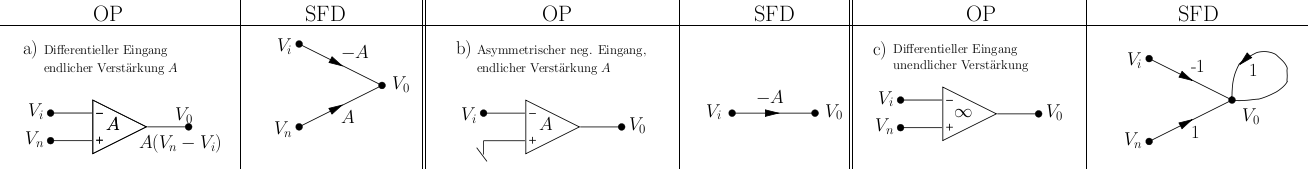
\includegraphics[width=18cm]{./bilder/sfd-op.png}

\subsection{Skalierung\formelbuch{245}}
	Um einen oder mehrere Knoten zu ändern, ohne das gesamte System zu
	ändern (Voraussetzung: Start/Endknoten werden nicht mitmaskiert), kann man
	diese Knoten skalieren.\\
	Vorgehen: 
	\begin{enumerate}
                \item Skalierungszone festlegen (Trennbündel)
                \item Alle eingehende Zweige mit $\lambda$ multiplizieren
                \item Alle ausgehende Zweige mit $\frac{1}{\lambda}$
                multiplizieren
    \end{enumerate}
    Wenn alle maximalen Signalniveaus gleich $\rightarrow$ maximal möglichen
    Dynamikbereich\\
    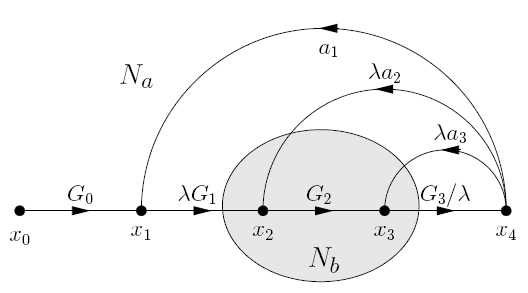
\includegraphics[width=7cm]{./bilder/sfd-scalierung.png}
    

